\documentclass{article}

% Language setting
% Replace `english' with e.g. `spanish' to change the document language
\usepackage[portuguese]{babel}

% Set page size and margins
% Replace `letterpaper' with `a4paper' for UK/EU standard size
\usepackage[letterpaper,top=2cm,bottom=2cm,left=3cm,right=3cm,marginparwidth=1.75cm]{geometry}

% Useful packages
\usepackage{amsmath}
\usepackage{graphicx}
\usepackage[colorlinks=true, allcolors=blue]{hyperref}

\title{Relatório do EP 3 de MAC0209}
\author{Andre Luis Neves, 15493840; Joao Victor Alonso de Mello, 10951790; Luis Vergara, 15472544}

\begin{document}
\maketitle


\begin{abstract}
  Nesse EP, nós medimos a frequencia do WiFi nos entornos do Instituto de Matemática e Estatística
  da Universidade de Sao Paulo (IME-USP). Usamos esses dados para gerar um mapa de calor (heatmap)
  no mapa do IME-USP. Além disso, geramos um video sobre a colecao de dados. 

Para o video, \href{https://youtube.com}{assistir no YouTube}.

\end{abstract}

\newpage

\tableofcontents

\newpage

\section{Introdução}
O WiFi é uma ferramenta essencial nas Universidades públicas brasileiras, e Universidades no geral.
Portanto, ter e manter uma boa frequencia e intensidade de sinal nos campus é de alta importância
tanto para os professores quanto para os alunos.  

Em particular, no IME-USP, há varios investimentos nos últimos anos que dependem de estudos e coleta
de dados para poder ser o mais eficientes possíveis. 

\section{Objetivos}
O objetivo principal desse projeto é coletar dados e processar eles para poder ter uma noção dos
pontos dos predios do IME-USP onde o sinal de WiFi é boa, e aqueles pontos onde há problemas de
conexão ou que tem baixa intensidade de sinal.  

% \section{Cronograma}

% Nesta seção, o grupo deve apresentar a Gantt Chartt de planejamento para o desenvolvimento do EP. Esta seção é a única obrigatória para o EP "Preparação do EP".

\section{Dados e métodos}
Nosso método principal de medição foi celulares smartphone juntamente com o aplicativo SideSeeing.
Mais informações sobre o aplicativo SideSeeing estão disponíveis no seguinte link:
https://arxiv.org/abs/2407.06464

Junto com outros colegas, caminhamos ao redor do prédio do IME-USP, tanto por fora quanto por
dentro, usando um colete com um smartphone que tem o aplicativo SideSeeing instalado nele. A coleta
de dados durou aproximadamente 2 horas.  

\section{Resultados experimentais}
Ver Figuras 1,2,3.  

\begin{figure}
  \begin{center}
    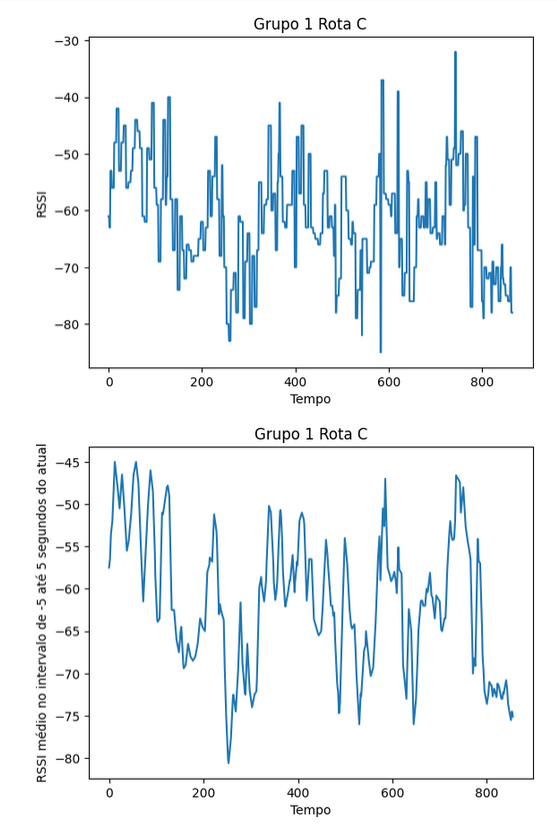
\includegraphics[width=0.95\textwidth]{figures/grupo_1-rota_c}
  \end{center}
  \caption{Grupo 1 Rota C}\label{fig:grupo_1-rota_c}
\end{figure}

\begin{figure}
  \begin{center}
    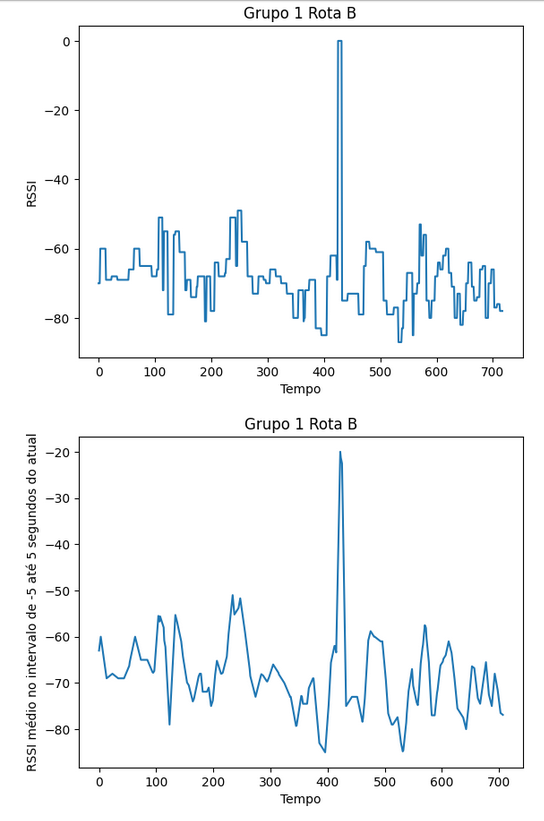
\includegraphics[width=0.95\textwidth]{figures/grupo_1-rota_b}
  \end{center}
  \caption{}\label{fig:}
\end{figure}

\begin{figure}
  \begin{center}
    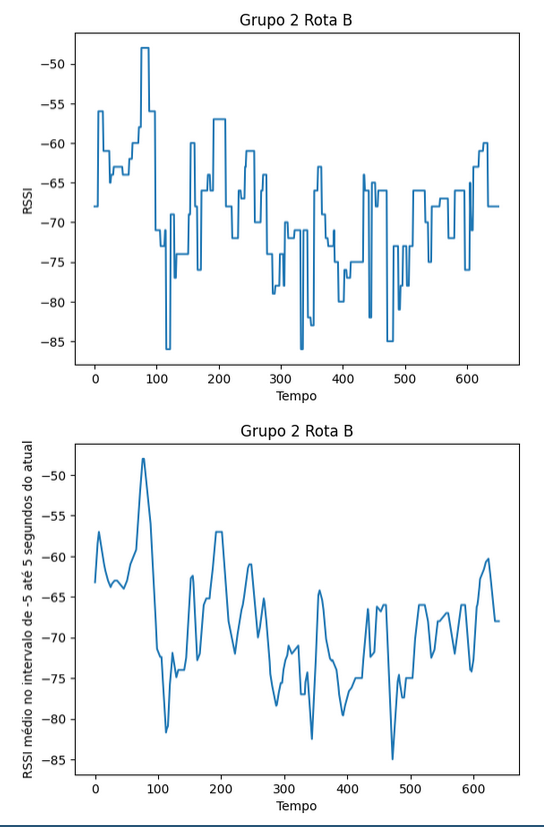
\includegraphics[width=0.95\textwidth]{figures/grupo_2-rota_b}
  \end{center}
  \caption{}\label{fig:}
\end{figure}


\section{Discussão e Conclusão}
A intensidade de sinal de WiFi dentro dos predios do IME-USP é maior nas salas de aula, um pouco
menor nos corredores, e menor ainda nas areas externas dos predios. 

\end{document}
